\documentclass[11pt]{article}

%------------------------------
% PREÁMBULO
%------------------------------

% PAQUETES

\usepackage{adjustbox}
\usepackage{amsmath}
\usepackage{apacite}
\usepackage[english,spanish,es-tabla]{babel}
\usepackage{booktabs}
	\renewcommand{\arraystretch}{1.25}
\usepackage{caption} 
	\captionsetup[table]{skip=10pt, width=.8\linewidth}
\usepackage{float}
	\setlength{\intextsep}{30pt}
\usepackage[T1]{fontenc}
\usepackage[bottom]{footmisc}
\usepackage[a4paper, margin=2cm]{geometry}
%	\geometry{
%	a4paper,
%	left=3cm,
%	right=4cm,
%	top=3cm,
%	bottom=3cm,
%	marginpar=3.4cm
%	}
\usepackage{graphicx}
	\graphicspath{ {figuras/} }
\usepackage[utf8]{inputenc}
\usepackage{lipsum}
\usepackage{lscape}
\usepackage{makecell}
\usepackage[round]{natbib}
%\usepackage{parskip}
\usepackage{setspace}
	\setstretch{1.5}
\usepackage[flushleft]{threeparttable}
%\usepackage[colorinlistoftodos]{todonotes}
\usepackage{xcolor}

% Paquete hyperref se carga al final antes de comenzar el documento (para evitar conflictos)
\usepackage{hyperref}
	\hypersetup{
		colorlinks=true,
		citecolor=blue,
		filecolor=blue,
		linkcolor=blue,      
		urlcolor=blue,
	}

\makeatletter
\newcommand{\myparagraph}[1]{\paragraph{#1}\mbox{}}
\makeatother


%------------------------------
% COMIENZA DOCUMENTO
%------------------------------


\begin{document}
	
	% TÍTULO
	
	% Cambiar footnote a símbolo para los thanks
	\renewcommand{\thefootnote}{\fnsymbol{footnote}}
	\setcounter{footnote}{1}
	
	\title{Notas sobre actividad I}

	\author{Desarrollo y Bienestar}

	\date{Curso 2019}
	
	\maketitle
	
	\noindent En la actividad del día 29/8/19 se presentó evidencia sobre el modelo de crecimiento chino. Como vimos, este país resulta interesante dado su acelerado y sostenido crecimiento a partir de su transición desde un sistema de planificación central hacia uno de mercado, con una fuerte participación del Estado en la actividad económica y el surgimiento de la empresa privada. \newline
	
	En el análisis vimos la evolución del PIB, PIB per cápita, evolución de la estructura productiva (agro, industria y servicios) y otras medidas que nos podían ayudar a entender las claves de este crecimiento. \newline
	
	Para completar el análisis, es interesante ver qué pasó en términos de distribución de riqueza. Algunas medidas que nos pueden ayudar a evaluar estos aspectos son el índice de Gini (visto en clase) y la tasa de pobreza (pueden buscar el Índice de Desarrollo Humano también si les interesa). Tener en cuenta que los conceptos aquí presentados no serán evaluados así que ¡tranquilos!
	
	\section{Índice de Gini}
	
	\begin{figure}[H]
		\centering
		\begin{minipage}{.8\textwidth}
			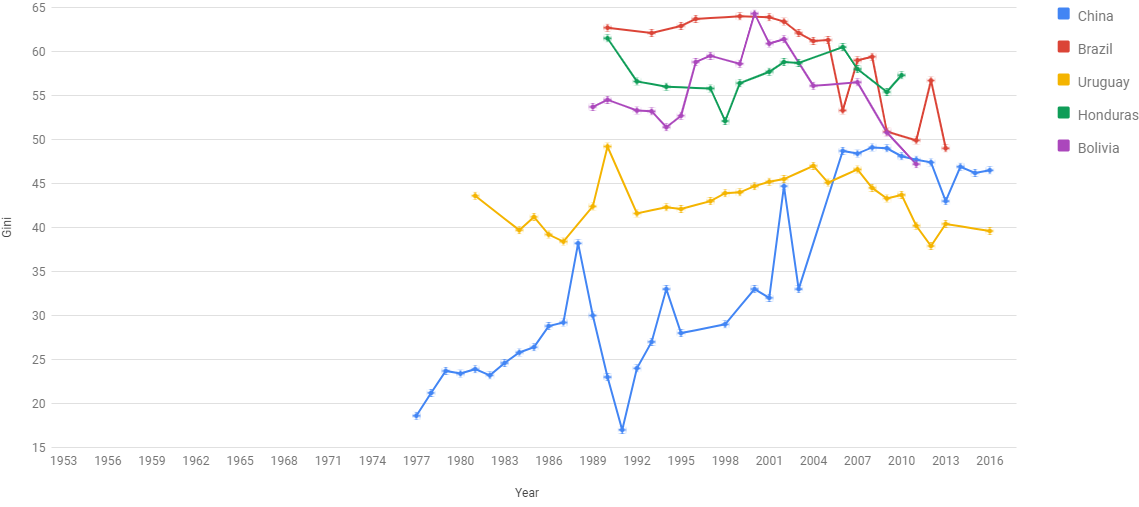
\includegraphics[width=\textwidth]{gini}
			{\footnotesize Fuente: World Income Inequality Database\par}
		\end{minipage}
		\caption{Evolución del Índice de Gini para varios países}
	\end{figure}
	
	\noindent El índice de Gini es el coeficiente de Gini multiplicado por cien, por lo que el rango del índice va de 0 a 100, siendo 0 perfecta igualdad y 100 perfecta desigualdad. ¿Qué puede interpretar del gráfico anterior? 
	
	\section{Tasa de pobreza}
	
	\noindent La medición más frecuente de pobreza unidimensional es la tasa de pobreza medida en términos de ingresos. Esta tasa mide la proporción de personas en un país con ingreso por debajo de línea de pobreza. Para definir la línea de pobreza se calcula el costo de una canasta de consumo básico alimentaria (que como indica su nombre incluye alimentos como pan, arroz, carne, frutas, verduras, etc.) más el costo de una canaste de consumo no alimentaria (que incluye bienes como calzado, medicamentos, artículos de higiene, etc.) \newline
	
	Otra medición utilizada es la tasa de indigencia. Esta tasa al igual que la anterior, define una línea de ingresos que se conoce como línea de indigencia. A diferencia de la línea de pobreza, la línea de indigencia sólo toma en cuenta el costo de la canasta básica alimentaria, por lo que mide la pobreza extrema. Es decir, la proporción de personas que se encuentran por debajo del ingreso necesario para cubrir los requerimientos nutricionales diarios básicos. \newline
	
	La forma en que se contruyen este tipo de medidas así como la composición de las canastas suele variar de un país a otro, por lo que la comparación internacional suele ser dificil. No obstante, determinados organismos internacionales como el Banco Mundial construyen indicadores basados en la definición de un umbral monetario único que se utiliza para todos los países.\newline
	
	A continuación se muestra la evolución de la pobreza utilizando el umbral de US\$ $1,90$ por día que calcula el Banco Mundial. Este umbral se calcula en función de los umbrales de pobreza que están definidos para los países más pobres del mundo. Por lo tanto, es una medida bastante restrictiva y se aproxima más a la indigencia (o pobreza extrema) que a la pobreza respecto a como se mide en Uruguay y otros países de ingreso medio como el nuestro. ¿Qué conclusiones puedes extraer al respecto?
	
	\begin{figure}[H]
		\centering
		\begin{minipage}{.8\textwidth}
			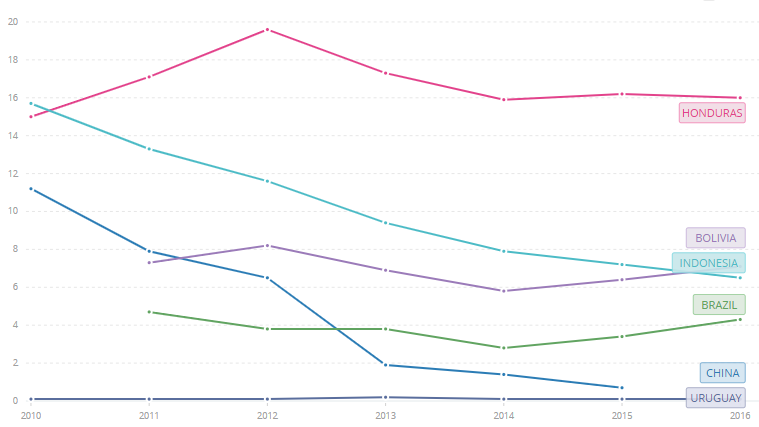
\includegraphics[width=\textwidth]{pobreza}
			{\footnotesize Fuente: Banco Mundial\par}
		\end{minipage}
		\caption{Evolución del Índice de pobreza US\$ 1,90 por día (2011 PPP)}
	\end{figure}
\end{document}